\documentclass[a4paper,12pt]{article}
\usepackage[
    a4paper, bindingoffset=0.2in, left=5mm, right=5mm, 
    top=30mm, bottom=18mm, footskip=5.5mm, headheight=15mm
]{geometry}
\usepackage{amsmath, accents, graphicx, caption, siunitx, float, fancyhdr}
\usepackage[bookmarks]{hyperref}
\newcommand*\rfrac[2]{{}^{#1}\!/_{#2}}
\newcommand{\im}[1]{j\; #1} 
\newcommand{\parallelTwo}[2]{\left.#1\,\middle/\!\middle/\,#2\right.}

\newcommand{\mR}[1]{\SI{#1}{\kilo\ohm}}
\newcommand{\mI}[1]{\SI{#1}{\milli\ampere}}
\newcommand{\mIu}[1]{\SI{#1}{\micro\ampere}}
\newcommand{\mV}[1]{\SI{#1}{\volt}}

% ------------ Header and Footer --------------------
\pagestyle{fancy}
\lhead{
\includegraphics[height=15mm]{./imagenes/Logo_UTN.png}}
\chead{
    \textsc{Electrónica Aplicada I} \\
    \footnotesize {Departamento de Electrónica} \\
    \footnotesize {Trabajo Práctico de Laboratorio. Período Lectivo 2019}
}
\rhead{}
\lfoot{ 
    \small{\textit{Grupo:}} \\
    \footnotesize{\textsc{Sukanec, Sanahuja, Caprula, Viña, Ortolan}}
}
\cfoot{}
\renewcommand{\footrulewidth}{0.4pt}% default is 0pt
\rfoot{\small{Pag \thepage}}


% ---------------------- Inicio Documento -------------------
\begin{document}
%%%%%%%%%%%%%%%%%%%%%%%%%%%%%%%%%%%%%%%%%
% Academic Title Page
% LaTeX Template
% Version 2.0 (17/7/17)
%
% This template was downloaded from:
% http://www.LaTeXTemplates.com
%
% Original author:
% WikiBooks (LaTeX - Title Creation) with modifications by:
% Vel (vel@latextemplates.com)
%
% License:
% CC BY-NC-SA 3.0 (http://creativecommons.org/licenses/by-nc-sa/3.0/)
% 
% Instructions for using this template:
% This title page is capable of being compiled as is. This is not useful for 
% including it in another document. To do this, you have two options: 
%
% 1) Copy/paste everything between \begin{document} and \end{document} 
% starting at \begin{titlepage} and paste this into another LaTeX file where you 
% want your title page.
% OR
% 2) Remove everything outside the \begin{titlepage} and \end{titlepage}, rename
% this file and move it to the same directory as the LaTeX file you wish to add it to. 
% Then add \input{./<new filename>.tex} to your LaTeX file where you want your
% title page.
%
%%%%%%%%%%%%%%%%%%%%%%%%%%%%%%%%%%%%%%%%%

%----------------------------------------------------------------------------------------
%	PACKAGES AND OTHER DOCUMENT CONFIGURATIONS
%----------------------------------------------------------------------------------------

% \documentclass[11pt]{article}
% \usepackage[utf8]{inputenc} % Required for inputting international characters
% \usepackage[T1]{fontenc} % Output font encoding for international characters
% \usepackage{mathpazo, graphicx} % Palatino font
% \begin{document}

%-------------------------------- TITLE PAGE -----------------------------------	
\begin{titlepage} % Suppresses displaying the page number on the title page and the subsequent page counts as page 1
	\newcommand{\HRule}{\rule{\linewidth}{0.5mm}} % Defines a new command for horizontal lines, change thickness here
	\center % Centre everything on the page
	
	%------------------- Headings -----------------------------
	\textsc{\LARGE Universidad Tecnológica \\[5pt] de Buenos Aires}\\[1.5cm] % Main heading such as the name of your university/college
	\textsc{\Large Electrónica Aplicada I}\\[0.5cm] % Major heading such as course name
	\textsc{\large Trabajo Práctico de Laboratorio Nº 2}\\[0.5cm] % Minor heading such as course title
	
	%-------------------- Title ----------------------------
	\HRule\\[0.4cm]
	{\huge\bfseries Amplificadores \\[5pt] Diferenciales }\\[0.4cm] % Title of your document
	\HRule\\[1.5cm]
	
	%-------------------- Author(s) ----------------------------
	\begin{minipage}{0.5\textwidth}
		\begin{flushleft}
			\large
			\textit{Integrantes}	\\[5pt]
			\begin{tabular}{ll}
				\textsc{Andes Sukanec} 	& \small{(Dirección)} 		\\[2pt] 
				\textsc{Juan Sanahuja} 	& \small{(Cálculos)} 		\\[2pt] 
				\textsc{Franco Caprula} & \small{(Mediciones)} 		\\[2pt]
				\textsc{Facundo Viña} 	& \small{(Simulación)}  	\\[2pt]
				\textsc{Javier Ortolan} &							\\[2pt]
			\end{tabular}			
		\end{flushleft}
	\end{minipage}
	~
	\begin{minipage}{0.4\textwidth}
		\begin{flushright}
			\large
			\textit{Profesor}\\
			\textsc{Ing. Daniel Pellettieri} % Supervisor's name
			\\[20pt]
			\textit{Ayudante}\\
			\textsc{Ing. Alejandro Gonzalez} % Supervisor's name
		\end{flushright}
	\end{minipage}
	
	% If you don't want a supervisor, uncomment the two lines below and comment the code above
	%{\large\textit{Author}}\\
	%John \textsc{Smith} % Your name
	
	%----------------- Date --------------------------
	\vfill\vfill\vfill % Position the date 3/4 down the remaining page
	{\large Noviembre 23 de 2019} % Date, change the \today to a set date if you want to be precise

	%------------------- Logo -----------------------------
	\vfill
	
\includegraphics[width=50mm]{./imagenes/Logo_UTN.png}\\[1cm] % Include a department/university logo - this will require the graphicx package
\end{titlepage}

% \end{document}


\section{Introduccion}
    Se planteo como objetivo lograr el diseño de un amplificador monoetapa con una resistencia de entrada decente
    y cuya ganancia fuera de entre 4 y 5 veces. 
    La resistencia de la señal se planteo como $\SI{50}{\ohm}$, valor típico de las fuentes de laboratorio.
    \\ \\
    Para satisfacer las necesidades impuestas se decidio por el diseño de un $R_E$ sin puentear. 
    \\ \\
    Al diseñar el circuito se trató al mismo tiempo de reducir el valor de la fuente de alimentación necesaria lo maximo
    posible. Por esto, y teniendo cuenta los dispositivos que se encontraban a nuestro alcance, se decidio por utilizar
    un transistor NPN BC337. 
    \\ \\
    Luego del diseño, en el cual se trato de imponer una $I_C \approx \mI{1}$, una $Av \approx 5$ y una $V_{cc} = \mV{3}$, 
    se obtuvo el siguiente circuito: 

\newpage
\section{Calculos}

\subsection{Estatico}
    A partir de la hoja de datos del BJT BC337 obtuvimos:
    \begin{itemize}
        \item $h_{FE} = 300$
        \item $V_{BE} = \mV{0.6}$
        \item $V_A = \mV{-100}$
    \end{itemize}

    Planteando Thevenin en la base del transitor se obtiene el siguiente circuito:
    % insertar circ estatico con RB
    Donde:
    \begin{gather*}
        V_{TH} = V_{CC} \cdot \cfrac{R_2}{R_1 + R_2} 
            = \mV{3} \cdot \cfrac{\mR{2.2}}{\mR{5.6} + \mR{2.2}} = \mV{0.85}
        \\ \\
        R_B = \parallelTwo{R_1}{R_2} = \parallelTwo{\mR{2.2}}{\mR{5.6}} = \mR{1.58}
    \end{gather*}

    A partir de esta equivalencia podemos despejar $I_B$ como:
    \begin{gather*}
        V_{TH} - I_B R_B - V_{BE} - I_E R_E = \mV{0} \\
        V_{TH} - V_{BE} - I_B ( R_B + (h_{FE}+1) R_E ) = \mV{0} \\
        I_B = \cfrac{V_{TH} - V_{BE}}{R_B + ( h_{FE}+1 ) R_E} 
            = \cfrac{ \mV{0.85} - \mV{0.6} } { \mR{1.58} + (300+1) \mR{0.22} = \mIu{3.69} }
    \end{gather*}

    Y conociendo las caracteristicas del transistor:
    \begin{gather*}
        I_C = I_B h_{FE} = \mIu{3.69} \cdot 300 = \mI{1.11}
        \\ \\
        V_{CE} = V_{CC} - I_C R_C - (I_C + I_E) R_E \\
        V_{CE} = \mV{3} - \mI{1.11} \cdot \mR{1.2} - ( \mI{3.69} + \mI{1.11} ) \mR{0.22} = \mV{1.42}
    \end{gather*}


\subsection{Dinamico}
    Segun el punto Q calculado en el estatico:
    \begin{gather*}
        g_m = \SI{40}{\cfrac{1}{\volt}} \cdot I_C = \SI{40}{\cfrac{1}{\volt}} \cdot \mI{1.11} = \SI{44.4}{\cfrac{mA}{V}}
        \\ \\
        h_{ie} = \cfrac{h_{FE}}{g_m} = \cfrac{300}{\SI{44.4}{\cfrac{mA}{V}}} = \mR{6.76}
        \\ \\
        r_o = \cfrac{| V_A |}{I_C} = \cfrac{|\mV{-100}|}{\mI{1.11}} = \mR{90}
    \end{gather*}

    Y con estos valores podemos sacar las resistencias de entrada $R_i$ y de salida $R_o$ como:
    \begin{gather*}
        R_i = h_{ie} + (1+h_{FE}) R_E = \mR{6.76} + (1+300) \mR{0.22} = \mR{73}
        \\ \\
        R_{BT} = \parallelTwo{R_B}{R_S} = \parallelTwo{\mR{1.58}}{\mR{0.05}} = \mR{0.05}
        \\ \\
        R_o = \big( \parallelTwo{(R_{BT} + h_{ie})}{R_E} \big) + r_o \bigg( 1 + \cfrac{h_{FE} R_E}{R_{BT} + h_{ie} + R_E} \bigg) \\
        R_o = \bigg( \parallelTwo{(\mR{0.05} + \mR{6.76})}{\mR{0.22}} \bigg) + 
            \mR{90} \cdot \bigg( 1 + \cfrac{300 \cdot \mR{0.22}}{\mR{0.05} + \mR{6.76} + \mR{0.22}} \bigg) \\
        R_o = \mR{0.21} + \mR{90} \cdot 10.39 = \mR{935}
    \end{gather*}

    Y segun el circuito dinamico podemos plantear la ganancia como:
    \begin{gather*}
        R_D = \parallelTwo{R_C}{R_L} = \parallelTwo{\mR{1.2}}{\mR{10}} = \mR{1.07}
        \\ \\
        A_v = \cfrac{v_o}{v_i} = \cfrac{ i_c \; (\parallelTwo{R_D}{R_o}) } { i_b R_i } 
            = \cfrac{ h_{FE} \; (\parallelTwo{R_D}{R_o}) } { R_i } \\
        A_v = \cfrac{ 300 \; (\parallelTwo{\mR{1.07}}{935}) } { \mR{73} } = 4.4
        \\ \\
        A_{vs} = A_v \; \cfrac{v_i}{v_s} = A_v \; \cfrac{R_B}{R_B + R_S} = 4.4 \; \cfrac{\mR{1.58}}{\mR{1.58} + \mR{0.05}} = 4.26
    \end{gather*}


\newpage
\section{Simulacion}
    %Al no disponer del modelo exacto de spice para el BC337 las simulaciones se realizaron utilizando el modelo generico NPN 200. \\
    La curva de ganancia obtenida fue la siguiente:
    \begin{figure}[H]
		\centering
		\captionsetup{labelformat=empty}
		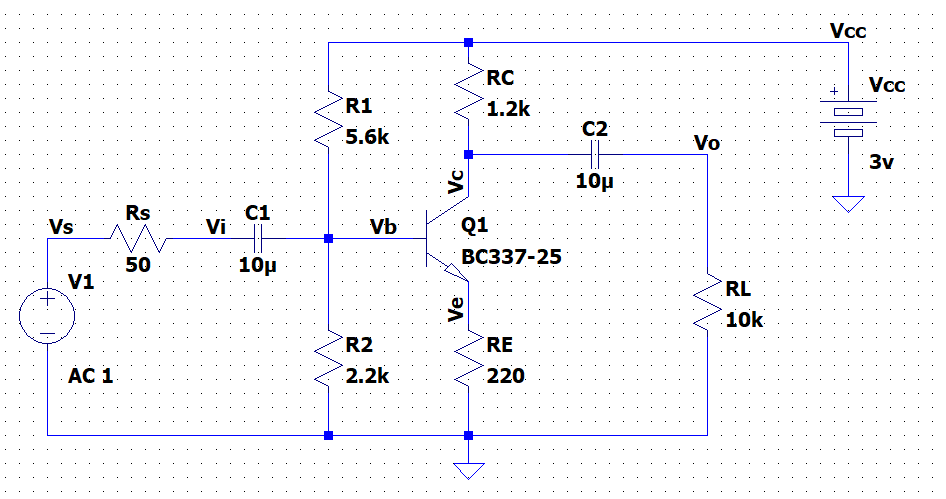
\includegraphics[height=80mm]{./imagenes/Circuito.png}
		\caption{\small{Circuito a simular}}
    \end{figure}
    \begin{figure}[H]
		\centering
		\captionsetup{labelformat=empty}
		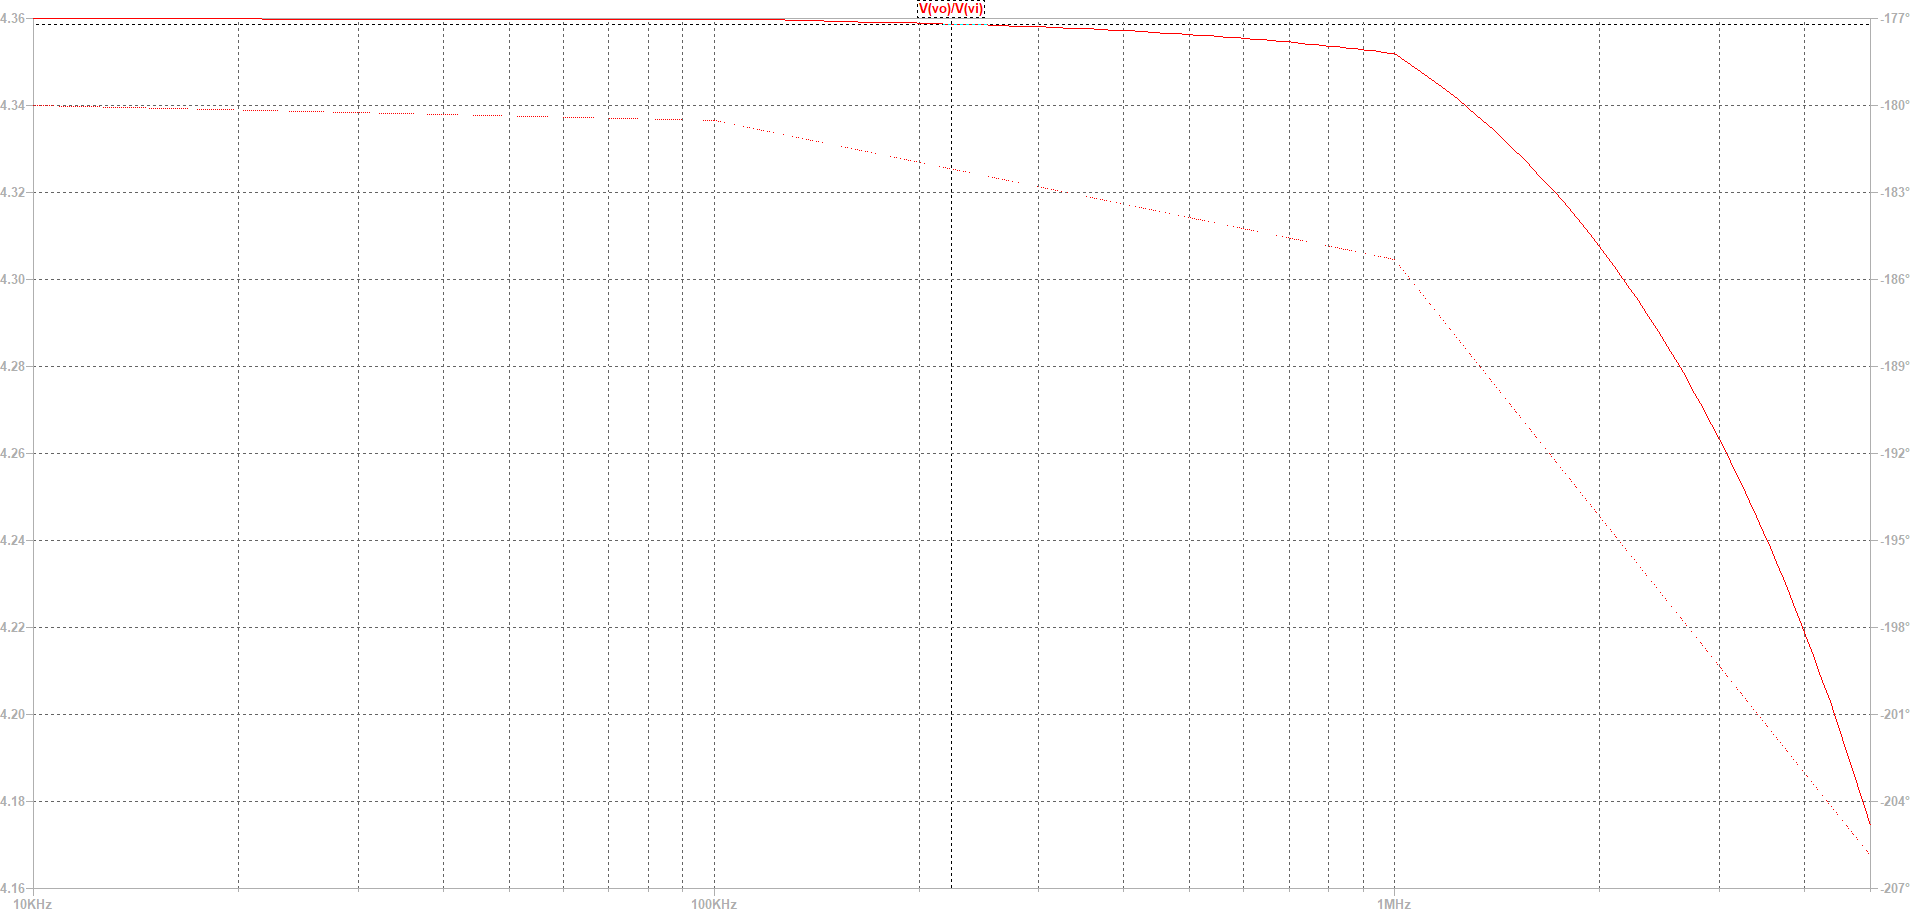
\includegraphics[height=80mm]{./imagenes/Curva_Ganancia.png}
		\caption{\small{Curva de ganancia}}
    \end{figure}

    El resto de los resultados se indican en la tabla presente en la siguiente seccion.


\newpage
\section{Cuadro de Resultados}

\subsection{Estatico}
\begin{table}[h]
    \centering
    \begin{tabular}{|c|c|c|c|}
        \hline
        Variable & Valor calculado      & Valor de simulacion & Valor medido      \\ \hline
        $V_{BEQ}$     & \mV{0.6}        & \mV{0.61}           & \mV{0.6}          \\ \hline
        $V_{CEQ}$     & \mV{1.42}       & \mV{1.52}           & \mV{1.39}         \\ \hline
        $I_{CQ}$      & \mI{1.11}       & \mI{1.04}           & \mI{1.15}         \\ \hline
        $V_{CBQ}$     & \mV{0.82}       & \mV{0.9}            & \mV{0.8}          \\ \hline
        $A_v$         & 4.4             & 4.36                & 4.4               \\ \hline
        $A_{vs}$      & 4.26            & 4.22                & 4.3               \\ \hline
    \end{tabular}
\end{table}

\subsection{Dinamico}
\begin{table}[h]
    \centering
    \begin{tabular}{|c|c|c|c|}
        \hline
        Capacitores     & f (\SI{}{\kilo\hertz})    & Vs (mV)   & Vo (V)    \\ \hline
                                & 1    & 100 & 0.43  \\ \cline{2-4}
                                & 10   & 100 & 0.43  \\ \cline{2-4}
                                & 20   & 100 & 0.42  \\ \cline{2-4}
                                & 50   & 100 & 0.42 \\ \cline{2-4}
                                & 100  & 100 & 0.41  \\ \cline{2-4}
                                & 200  & 100 & 0.41  \\ \cline{2-4}
        \SI{10}{\micro F}       & 300  & 100 & 0.41  \\ \cline{2-4}
                                & 400  & 100 & 0.40   \\ \cline{2-4}
                                & 800  & 100 & 0.39  \\ \cline{2-4}
                                & 1000 & 100 & 0.38  \\ \cline{2-4}
                                & 1500 & 100 & 0.33  \\ \cline{2-4}
                                & 2000 & 100 & 0.28  \\ \cline{2-4}
                                & 3000 & 100 & 0.21  \\ \cline{2-4}
                                & 4000 & 100 & 0.18  \\ \cline{2-4}
                                & 5000 & 100 & 0.15  \\ \hline
    \end{tabular}
    \quad
    \begin{tabular}{|c|c|c|c|}
        \hline
        Capacitores     & f (\SI{}{\kilo\hertz})    & Vs (mV)   & Vo (V)    \\ \hline
                                & 1    & 100 & 0.44  \\ \cline{2-4}
                                & 10   & 100 & 0.43  \\ \cline{2-4}
                                & 20   & 100 & 0.42  \\ \cline{2-4}
                                & 50   & 100 & 0.41 \\ \cline{2-4}
                                & 100  & 100 & 0.40  \\ \cline{2-4}
                                & 200  & 100 & 0.40  \\ \cline{2-4}
        \SI{100}{\micro F}      & 300  & 100 & 0.40  \\ \cline{2-4}
                                & 400  & 100 & 0.40   \\ \cline{2-4}
                                & 800  & 100 & 0.38  \\ \cline{2-4}
                                & 1000 & 100 & 0.35  \\ \cline{2-4}
                                & 1500 & 100 & 0.30  \\ \cline{2-4}
                                & 2000 & 100 & 0.26  \\ \cline{2-4}
                                & 3000 & 100 & 0.22  \\ \cline{2-4}
                                & 4000 & 100 & 0.18  \\ \cline{2-4}
                                & 5000 & 100 & 0.15  \\ \hline
    \end{tabular}
\end{table}
\begin{table}[h]
    \centering
    \begin{tabular}{|c|c|c|}
        \hline
        Variable    & Valor calculado   & Valor medido      \\ \hline
        $R_i$       & $\mR{73}$         &                   \\ \hline
        $R_o$       & $\mR{935}$        &                   \\ \hline
    \end{tabular}
\end{table}


\newpage
\section{Conclusiones}
    Al momento de armar el circuito se noto que este era muy sensible a los cambios en la tensión base emisor $V_{BE}$. 
    Si bien esto no se habia tenido en cuenta, se propuso que esto era un mal necesario para satisfacer la necesidad de una fuente
    de alimentacion de tan solo \mV{3}. 
    \\ \\
    Siguiendo esta problemática es que durante la práctica nos encontramos con que el valor de $V_{BE}$ era de \mV{0.6}, contrario a los
    \mV{0.7} que se habian planteado originalmente al momento del diseño. Por esto mismo es que se tomó la decisión de modificar la
    resistencia $R_2$ de manera que se mejorara la excursión resultante (el valor original de la misma era de \mR{2.7}).
    \\ \\
    Finalmente se comprobó lo dicho ya varias veces durante la materia, que la única manera de diseñar circuitos con salidas estables
    independientemente de las variaciones de sus componentes es por medio de realimentaciones.

\end{document}
